\documentclass[../main.tex]{subfiles}
\graphicspath{{\subfix{../images/}}}

\begin{document}

\begin{newrequirements}
    \begin{todolist}
        \item detailed design specifications of the 
            hardware and software to meet the 
            functional requirements and the 
            practical design constraints 

        \item use circuit diagrams, logic diagrams, 
            block diagrams, flow charts, class 
            diagrams and/or sequence diagrams 

        \item detailed justification of design 
            choices 

        \item highlight the novel design aspects 

        \item evaluate the effect of design choices 
            on your system quality attributes 

        \item not required to include all of these 
            sub-sections, instead you need to 
            decide how to best communicate your 
            solution’s design
    \end{todolist}
\end{newrequirements}

\subsection{Overview}

% \begin{newrequirements}
%     \begin{todolist}
%         \item a simple one or two paragraphs giving a 
%             birds-eye view of the solution 

%         \item very generic so that even a layman will 
%             be able to comprehend the scope of your 
%             work 

%         \item a high level architecture diagram of 
%             the proposed solution. The diagram 
%             should show how your solutions is 
%             decomposed and organized into 
%             components. Can be a Block Diagram or 
%             Illustrative Block diagram in which 
%             some components/blocks can be 
%             illustrations/images of the actual 
%             component. 

%         \item Describe the role and the interfaces of 
%             key components of your high level 
%             architecture. 

%         \item Discuss the key interactions between 
%             the identified components. 

%         \item While one Block diagram can be used to 
%             show hardware components/connectivity, 
%             another Block diagram or Flow chart can 
%             be used to do the same for the software 
%             aspect of the project. 
                
%     \end{todolist}
% \end{newrequirements}

The overview of the proposed solution is depicted in 
\cref{fig:solution-overview}. 
The hardware components consist of an \anafi drone,
a Raspberry Pi with an external battery, and a Wi-Fi
dongle. The built-in camera of the drone is used to
take pictures of the targets and the Wi-Fi dongle
is used to communicate with the command and control
system, which sends high-level commands whenever the
connection is present. An object detection model trained
using RoboFlow detects and identifies the targets in the
pictures. In addition, a \gls{drl} agent is trained 
in a cyber-physical simulator called Sphinx to
visit virtual targets having the same mobility pattern as the
real ones.
This finished model is loaded into the Raspberry Pi that acts
as an onboard computer to the \anafi drone and instructs
it where to move to cover the targets in a minimum amount
of time.

The following subsections will
explain in more detail why this solution is chosen
and what the integral components are.

\begin{figure}[tbp]
	\centering
	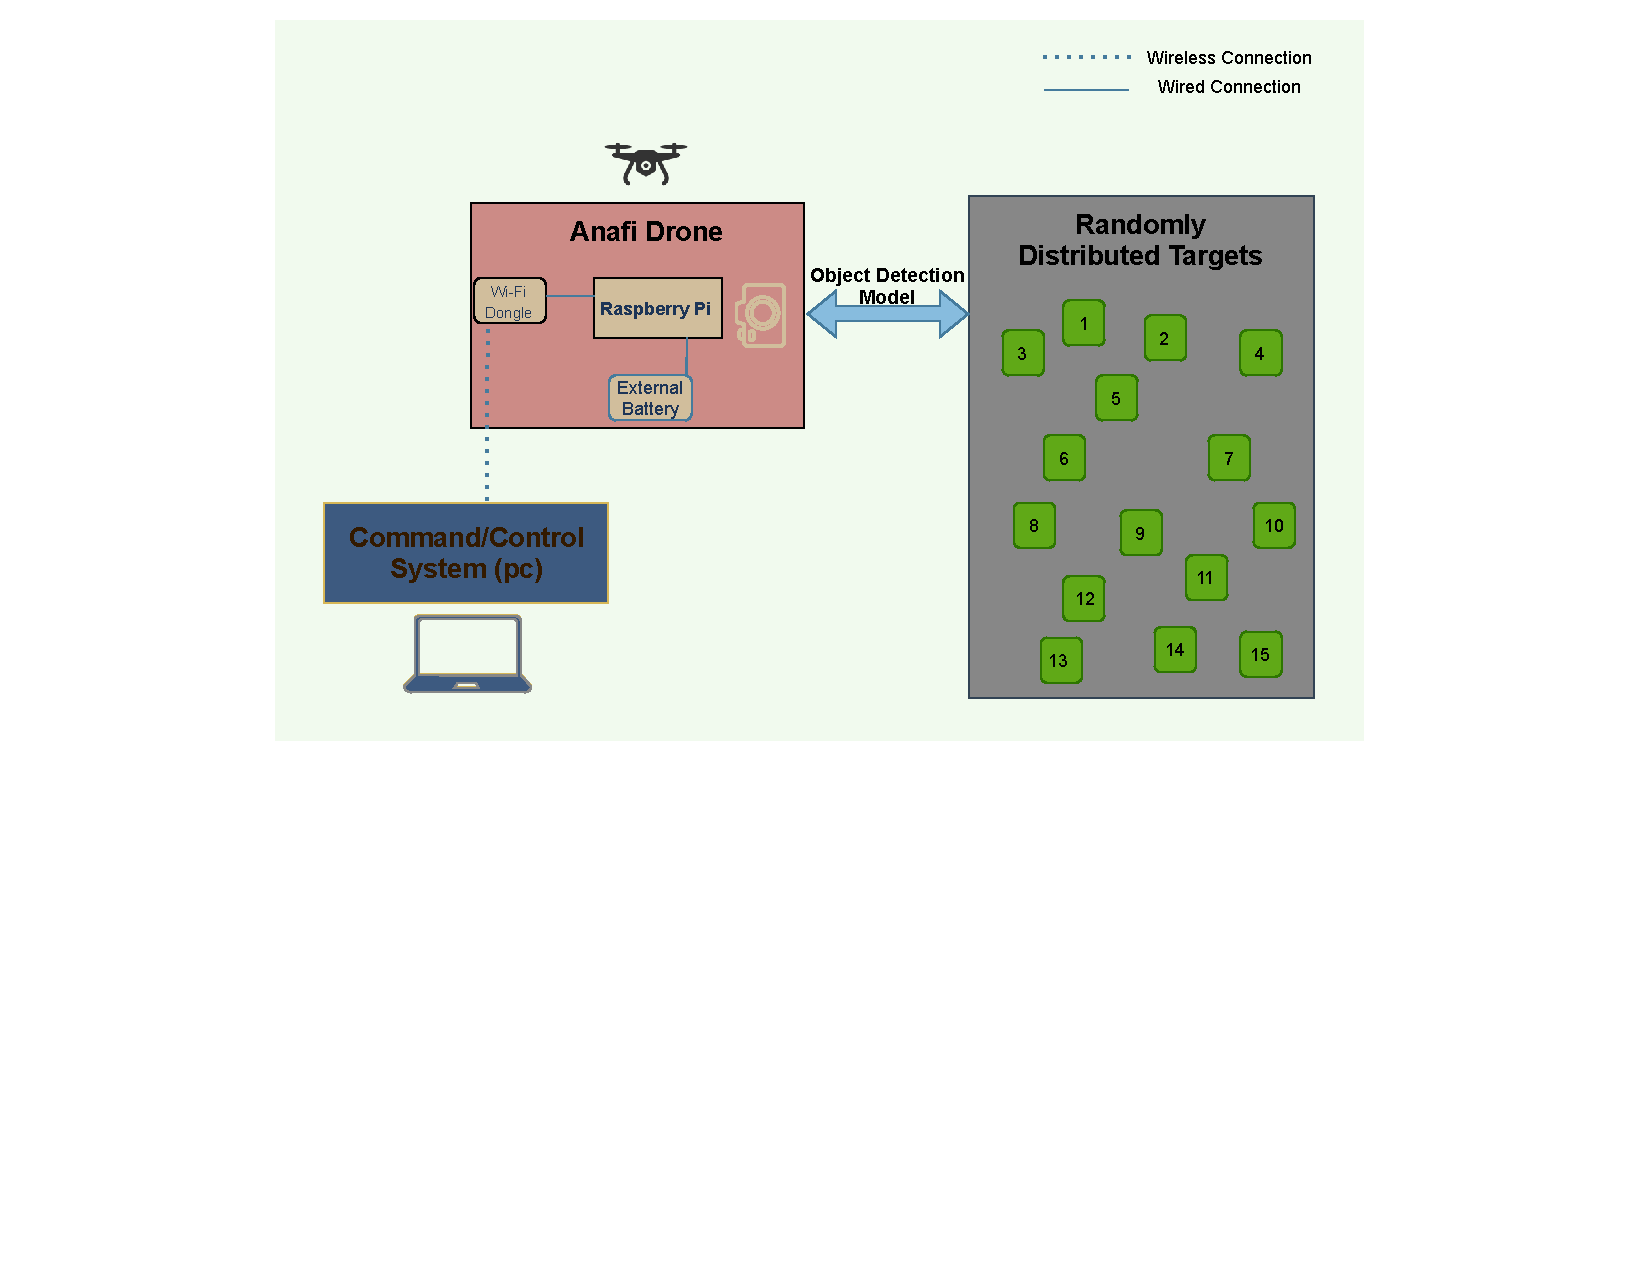
\includegraphics[width=0.9\textwidth]{solution-diagram}
	\caption{A general overview of the solution.}
	\label{fig:solution-overview}
\end{figure}

\subsection{High level architecture}

\Cref{fig:arch-fig} shows a high-level architecture 
of the complete working system, in which a group 
of connected adapters and devices are combined into 
a single functional system. 
The architecture is composed of three sections namely
interfacing, controlling, and targets. 
The interfacing section contains the drone that 
will handle the onboard computer, its power source, 
and the connection adapters. 
In the controlling part, a personal computer 
will be responsible for contacting the onboard computer 
to adjust settings, execute scripts, and get 
live updates and results. 
Finally, there are multiple moving targets 
in the target section. For example, 
\gls{rc} cars are controlled manually and move in 
a specific mobility pattern with varying directions 
and destinations. 
In the next section, hardware and software components 
will be presented in a more detailed manner.

\begin{figure}[tbp]
    \centering
    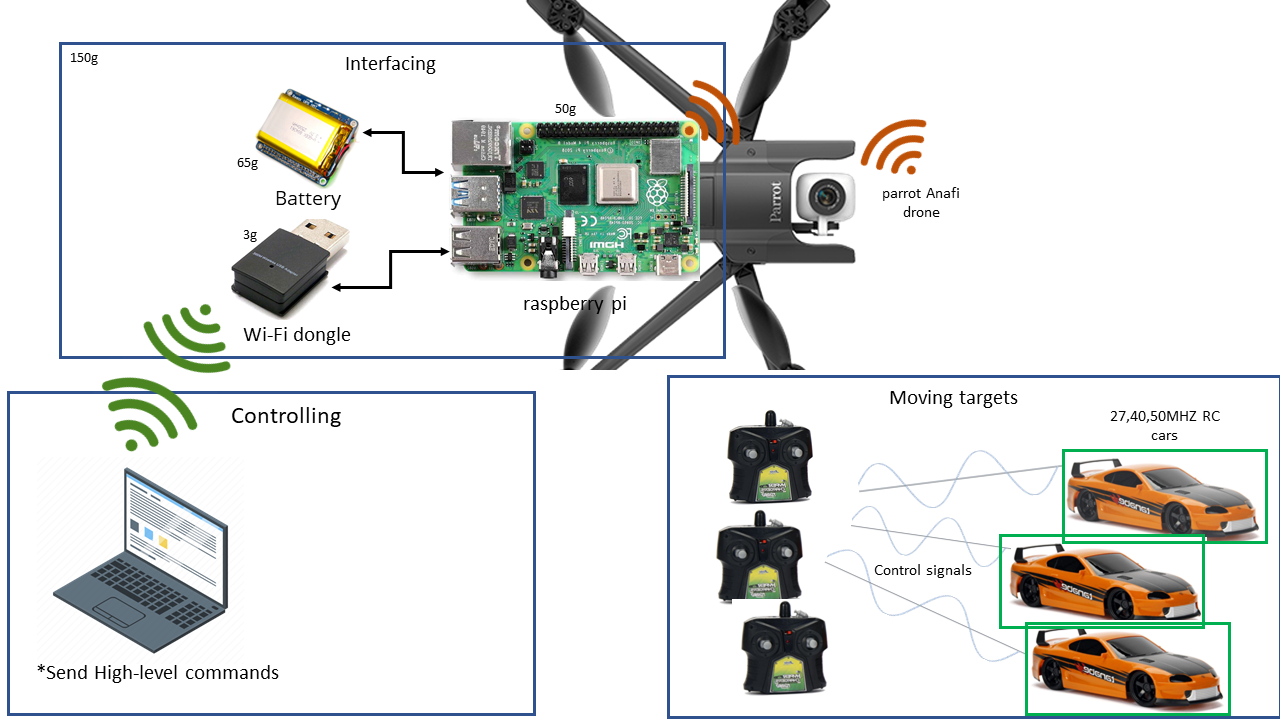
\includegraphics[width=0.9\textwidth]{high-level-arch.png}
    \caption{The high-level architecture of the overall system.}
    \label{fig:arch-fig}
\end{figure}

\subsection{Hardware/software used}

\begin{newrequirements}
    \begin{todolist}
    \item Describe each hardware component and how it works 
        and the \textbf{scientific principles of its 
        inner working}.
    \end{todolist}
\end{newrequirements}

\subsubsection{Software}

There are three primary categories of software 
depending on the usage: simulation, training, 
and application, and they are listed in \cref{tab:software-used}. The first part will focus on 
simulating the environment, testing the models, 
and flight control. Before discussing the software 
to be used, we have selected Ubuntu 18.04 (Bionic Beaver) 
as an operating system for several reasons. 
One key reason is that in addition to
still being supported, it is compatible with the 
Parrot's Olympe and Sphinx programs, which are only 
supported on limited distributions and operating systems.
Another reason is that it is a lite \textsc{os} 
and can be installed on the onboard computer that 
will be attached to the drone. For the simulation part, 
using Sphinx and Gazebo software is very helpful
to visualize the environment, control the drone, 
and apply the \gls{drl} model. 

\begin{table}[p]
    \centering
    \caption{Software used in the project.}
    \label{tab:software-used}  
    \begin{tabular}{ p{3cm} p{3cm} p{6cm} }
        \toprule
        \textit{Software} 
            & \textit{Logo} 
                & \textit{Justification} \\ 

        \midrule

        Parrot Olympe  
            & 
            \raisebox{-0.7\height}
            {
\includegraphics[width=2.7cm]
            {parrot.png}}
                & A controller for the Parrot \anafi 
                drone. It makes controlling 
                the drone possible 
                using a Python script \\
                \addlinespace

        Parrot Sphinx  
            & 
            \raisebox{-0.7\height}
            {
\includegraphics[width=2.7cm]
            {parrot.png}}
                & A simulator for the Parrot \anafi drone.
                It loads the Parrot's drone firmware 
                in the simulation environment.
                It is largely based on Gazebo. \\
                \addlinespace

        Roboflow  
            & 
            \raisebox{-0.9\height}
            {
\includegraphics[width=2.4cm]
            {roboflow.png}}
                & A framework for Computer Vision
                development that can be used online.
                It facilitates labelling of images, 
                splitting and merging datasets, 
                applying image transformations 
                and filters, 
                and generating a link for 
                the augmented datasets 
                which will be used in the 
                training notebooks.  \\
                \addlinespace

        Jupyter Notebook  
            & 
            \raisebox{-0.9\height}
            {
\includegraphics[width=2.5cm]{jupyter.png}}
                & A web application for writing, testing 
                and sharing of code. It is free 
                and does not require internet access like 
                the Google Colab. It is used heavily 
                in this project to experiment with new 
                ideas in the Sphinx simulation. \\ 
                \addlinespace

        Google Colab 
            & 
            \raisebox{-0.9\height}
            {
\includegraphics[width=2.8cm]{colab.png}}
                & A Jupyter notebook environment
                running in the cloud. 
                It makes it easy to write, run, 
                and share the code. Most importantly, 
                it gives an option to use remote 
                processing resources in addition to the 
                local ones. \\ 
                \addlinespace

        \bottomrule
    \end{tabular}
\end{table}

Sphinx is a simulation 
tool built on top of Gazebo 
to run the Parrot's drone firmware on 
personal computers, which comes with helpful 
features for simulation such as visualizing flight 
data at runtime, running the \gls{uav} remotely, 
and executing scripts with the command line. 
Gazebo is a robot \textsc{gui} simulation 
which simulates the visual and physical surrounding 
of drones and custom 3D objects. 
\Cref{fig:gazebo} shows how the Sphinx 
program looks like. 

\begin{figure}[tbp]
    \centering
    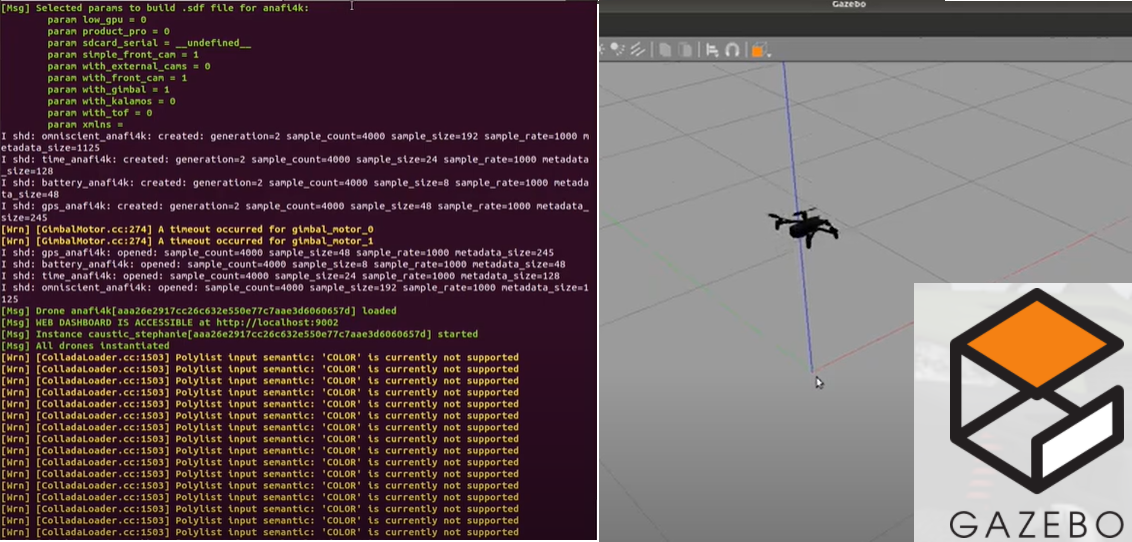
\includegraphics[width=0.9\textwidth]{gazebo.png}
    \caption{The Sphinx program that runs on top of Gazebo.}
    \label{fig:gazebo}
\end{figure}

The training part is divided into \gls{rl}, 
which is used to teach the \anafi drone to complete the task, 
and object detection and identification, 
which is used to detect and count the targets
required in determining the reward during the training. 
The \gls{rl} agent is based on the \gls{drl} model 
developed by \textcite{Ged21}. The action space is composed 
of 9 movements in the 
forward, backward, left,
right, forward-left, forward-right, backward-left and 
backward-right directions as well as a hover.
The state space is given as
\begin{align}
    s = \{ t, cell, [ I_1, I_2, I_3, \ldots, I_m] \} 
    \label{eq:state-space}
\end{align}

\noindent 
where $t$ is the current time step, $cell$ is the \id of the
cell above which the drone is, $I_k$ is the binary variable 
that indicates if the target with an \id of $k$ has been
visited, $m$ is the total number of targets,
and the vector of length $m$ is the container for the
$I$ indicators. 
For example,
if only targets with \id's 3 and 7 have been visited
in the current and previous time steps since the beginning of the 
episode,
then the vector will have elements of one for $I_3$ and $I_7$ while
the other elements are zeros.
It follows that all the targets must be uniquely identifiable.
In addition, the reward is how many new targets are captured 
in the current cell,
and if the drone flies past the boundary, then a big negative
reward will be incurred.

For the object detection, we used simulation tools to 
generate some training datasets. Firstly, 
we placed random objects and captured the images 
using the simulated drone camera. We have used a 
website called Roboflow which helped us labelling 
the objects and generate new datasets from the 
existing ones with different types of augmentation 
such as rotation and scaling. 
For the object detection model, Google Colab notebook 
was a sufficient tool to start training using 
\gls{cnn} \textsc{yolo}v5 in addition to the 
Jupyter notebook which was very helpful 
in code experimentation. 

For the application software, Parrot Olympe 
was used to send commands to the physical as well as 
the simulated drone and control the flight trip and 
how the drone moves. Parrot Olympe uses Python 
controller programming interface for Parrot drones 
which makes controlling simple and easy using a 
Python script. Moreover, Olympe allows us to read
sensor data, such as the \gls{gps} fixes and camera feed, 
from the \anafi
drone. This will make it possible to build a user interface
on the control and command station
shown in \cref{fig:ui-prototype} to monitor 
the progress of the drone
when it is autonomously executing the task visitation
mission.

\begin{figure}[tbp]
    \centering
    \includegraphics[width=0.9\textwidth]{ui-prototype}
    \caption{An example of a user interface that will be built
                using sensor data coming from the \anafi drone.}
    \label{fig:ui-prototype}
\end{figure}

\subsubsection{Hardware}

The main core of the hardware part is the drone, 
which will be the Parrot \anafi.
\Cref{tab:hardware-used} lists the hardware components
used in this project and their justifications. This quad-copter
drone is powerful because it combines many technologies 
and sensors in a small foldable size. It also it has 4K HDR Camera supported 
with 180 degree gimbal. 
There are seven sensors in total inside the drone which are shown in 
\cref{tab:sensors-table} 


\begin{table}[H]
	\centering
	\caption{Processor and sensors inside the drone}
	\label{tab:sensors-table}  
	\begin{tabular}{ p{4cm} p{8cm} }
		\toprule
		\textit{Part Name} 
		& \textit{used for}  \\ 
		
		\midrule
		Ambarella H22 
		processor
		& powerful Quad-core ARM® Cortex™ - capable of dealing with sensors and video I/O , 
		image processing , video encoding , interfacing \\ 
		3-axis gyroscope
		& measure the orientation and angular velocity  \\ 
		3-axis accelerometer
		& measure the acceleration in 3 dimensions  \\ 
		magnetometer 
		& measure the Earth's magnetic field to know the orientation and the heading   \\ 
				barometer 
		& measure atmospheric pressure change to control flight height   \\ 
				GPS 
		& determine the location of the drone and navigation  \\ 
				Ultrasonar 
		&  height measurement for small height less than 5 meters  \\ 
				Vertical camera 
		&  measuring horizontal speed and height using optical flow \\ 
        \bottomrule
    \end{tabular}
\end{table}   

The second important device is the Raspberry Pi 4 model B. It 
acts as an onboard computer and is used in this project
mainly to facilitate the low-level control of the drone
by sending frequent control commands to the drone
in a certain direction or stay hovering.
The choice of action is determined by the \gls{drl}
model that will be installed in it.
Hence, the tasks of the Raspberry Pi are: 

\begin{enumerate}
	\item connecting to the drone's access point 
	using a Wi-Fi interface,
	\item controlling the drone 
	by executing Olympe to send low-level control signals 
	and to receive sensory data,
	\item applying the \gls{drl} model supported by 
	the command and control system,
	\item receiving high-level commands and sending video 
	frames to the command-control system from the drone camera.
\end{enumerate}
 
The Parrot \anafi drone is connected 
to the Raspberry Pi, which is the onboard computer,
using both devices' internal 
\SI{2.4}{\giga\hertz}
Wi-Fi interfaces. 
Firstly, we add the \anafi drone's access point 
to the saved devices list in the Raspberry Pi.
Once the Raspberry Pi boots up, it automatically keeps 
searching for the access point and connects 
to it once it is available.

For the connection between the command and control system 
and the Raspberry Pi, 
the Raspberry Pi will use a 
\SI[per-mode=symbol,per-symbol=p]{300}{MBps} 
Wi-Fi adapter dongle connected to 
its \textsc{usb} port. 
This will allow it to create an access point to which 
the command and control device will connect and by which 
the Raspberry Pi can be controlled. This control of the 
onboard computer is done through the graphical user interface,
which is simply a web-based application 
that will allow the user to send the
control commands and receive the video frames. 


Regarding the power source for the Raspberry Pi, 
we considered taking power directly from the 
drone's battery, but after some research, we found 
that the \anafi drone's  
socket is somehow different in the type and the power output. It is also challenging 
because the drone battery is susceptible to shutting down 
immediately if the voltage reaches less than 3.0 Volt. 
Therefore, we did not want to take the risk so we used a 
lithium battery with a power board called 
\textsc{upsp}ack Standard Power Supply attached to 
the main Raspberry Pi board. It includes a 
\SI{4000}{\milli\ampere\hour}
lithium battery, which provides enough power 
and long-lasting time for our application.
\Cref{tab:hardware-used} lists the hardware components
used in this project and their justifications. 
\begin{table}[p]
	\centering
	\caption{Hardware used in the project.}
	\label{tab:hardware-used}  
	\begin{tabular}{ p{4cm} p{3cm} p{6cm} }
		\toprule
		\textit{Hardware} 
		& \textit{Picture} 
		& \textit{Justification} \\ 
		
		\midrule
		
		Parrot \anafi Drone  
		& \begin{minipage}{.1\textwidth}
			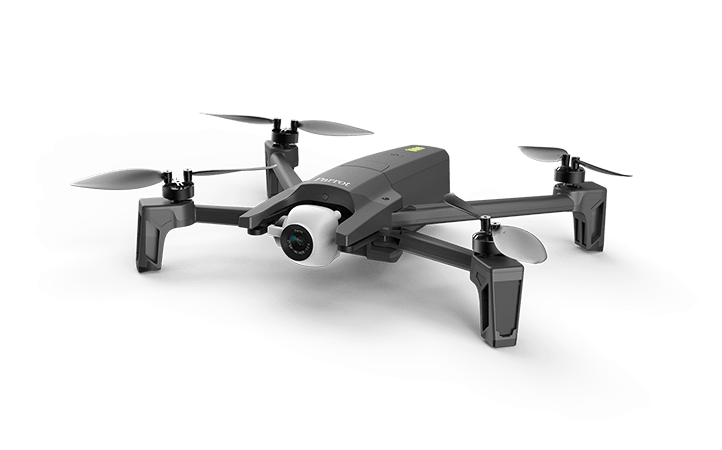
\includegraphics[width=30mm, height=20mm]{anafi.png}
		\end{minipage} 
		& Available in the university, can be 
		controlled easily 
		with simple Python script, 
		4K-high resolution camera.  \\ 
		\addlinespace
		
		Raspberry Pi 4  
		& \begin{minipage}{.0\textwidth}
			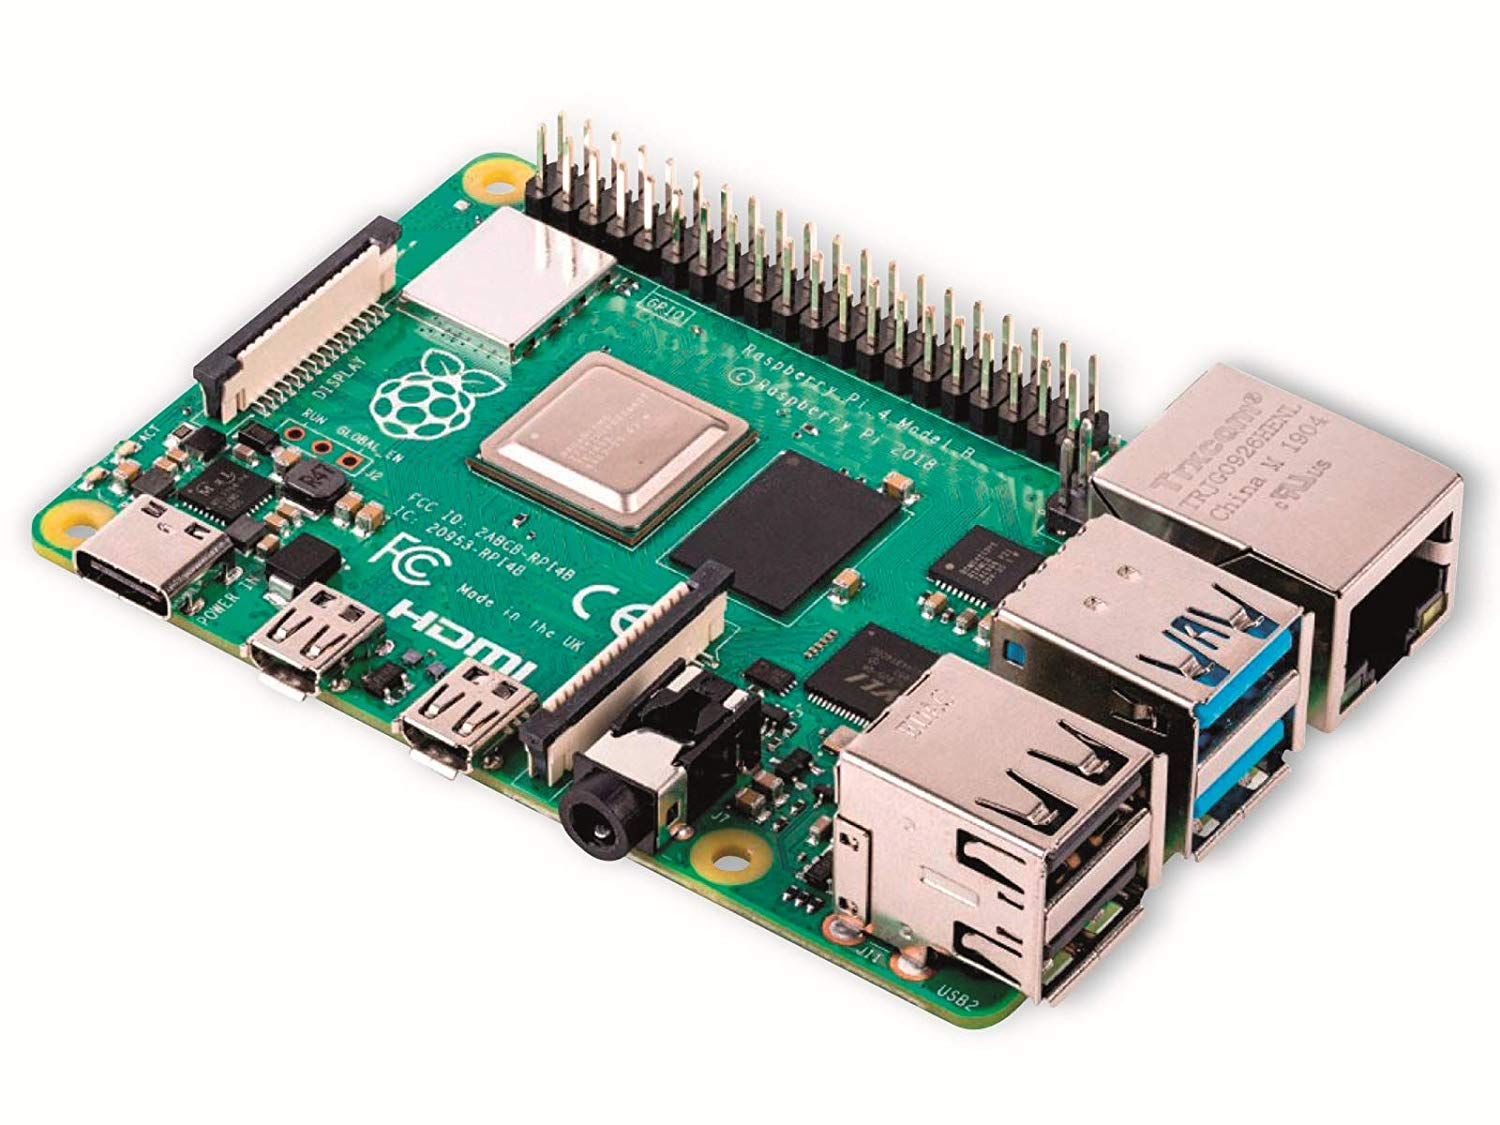
\includegraphics[width=30mm, height=20mm]{raspberry.jpg}
		\end{minipage} 
		& Specifications are enough for our 
		application, support Wi-Fi and its 
		small size and weight is an advantage.\\ 
		\addlinespace
		
		\textsc{rpi} \textsc{upsp}ack \textsc{v}3 with 
		\SI{4000}{\milli\ampere\hour} 
		lithium Battery  
		& \begin{minipage}{.1\textwidth}
			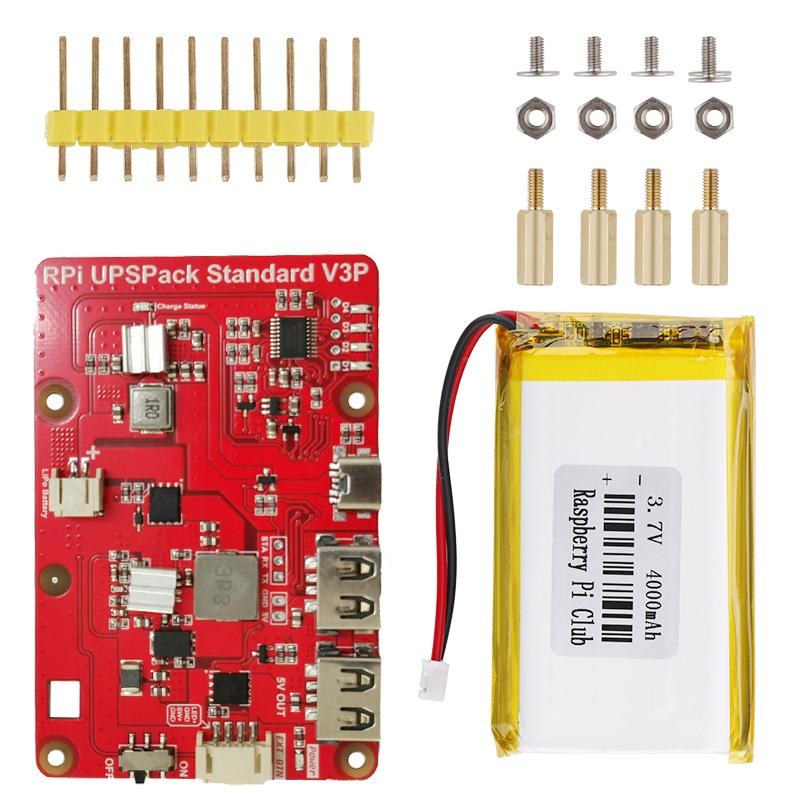
\includegraphics[width=30mm, height=35mm]{RPI.jpg}
		\end{minipage}  
		& Support up to 4 hours which is more 
		than enough , the board got an \textsc{led} 
		indicator for charging level also the 
		weight and shape is an advantage.  \\ 
		\addlinespace
		
		Wireless N Nano \textsc{usb} Adapter  
		& \begin{minipage}{.1\textwidth}
			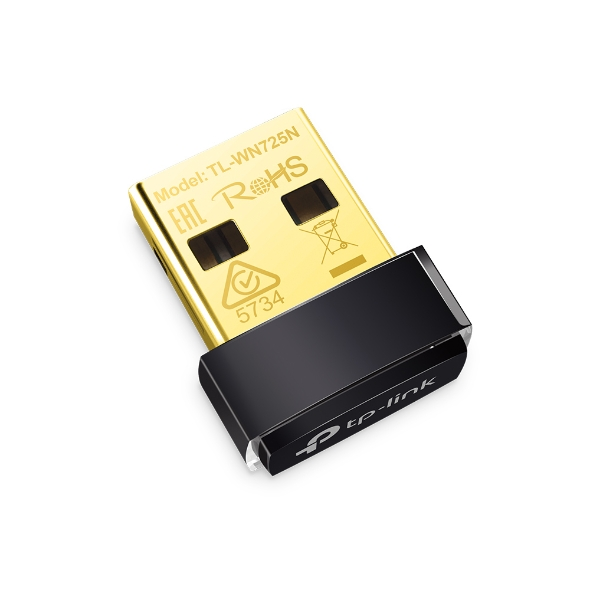
\includegraphics[width=28mm, height=28mm]{dongle.jpg}
		\end{minipage} 
		& Cheap and do its job, good coverage 
		range.  \\ 
		\addlinespace
		
		Laptop 
		& \begin{minipage}{.1\textwidth}
			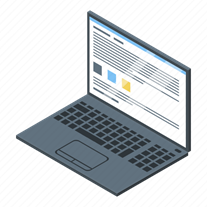
\includegraphics[width=30mm, height=30mm]{laptop.png}
		\end{minipage} 
		& Any laptop with good WiFi interface 
		card will be enough for our case. \\ 
		\addlinespace
		
		\bottomrule
	\end{tabular}
\end{table}


\subsection{Hardware design}

\begin{newrequirements}
    \begin{todolist}
        \item[\done] For major hardware subsystems in your 
            design, you must present the theory 
            behind the different technological 
            approaches, the tradeoffs associated 
            with each approach, and your 
            justification for selecting a 
            particular approach. For instance, 
            selection of a particular 
            microcontroller for your design; what 
            were the main factors that contributed 
            to this specific choice. For example, 
            you may choose between Arduino, 
            MC68HCxxx, BasicStamp, and PIC18Fxx and 
            you have decided to use PIC18F47 due 
            to: 

        \begin{todolist}
        \item its programming compatibility with C 

        \item its low cost 

        \item its development platform availability 

        \item ability to input analog signals 
        \end{todolist}

        \item To document the design of the hardware 
        components you can use as many of the 
        following as possible: 

        \begin{todolist}
        \item Circuit Diagram (Showing actual circuit 
        diagram with all the components used) 

        \item Connectivity diagram for modular 
        hardware. 

        \item Logic Diagrams (Showing logic flow with 
        respect to signals/numbers) 

        \item Functional Diagrams (showing subsets of 
        the circuit as functional blocks) 

        \item State Diagrams (to explain the 
        sequential logic flow) 

        \item Any other drawings to communicate your 
        design 
        \end{todolist}

        \item Organize the content of this section 
        using appropriate subsections. It is 
        recommended to have a sub-section of 
        each of the recommended artifacts 
        listed above. 

    \end{todolist}
\end{newrequirements}

\subsubsection{UAV options}
\begin{table}[H]
	\centering
	\caption{A comparison of the \gls{uav} options.}
	\label{tab:alt-solutions}
	\begin{tabularx}{\textwidth}{ p{4cm} X X }
		\toprule
		\textit{} & \textit{Option A} & \textit{Option B}\\ \midrule
		Type  & Custom made drone with onboard computer & 
		Commercial drone with high performance and many features    \\
		Flexibility & Very flexible and customization is easy & 
		Hard to customize or modify it since it flies under 
		limited protocols and standards. \\
		
		Price and Availability & Cheaper but the shipping and 
		building processes must be considered & Expensive but 
		in our case its available in our hands and ready to fly.   \\
		
		Onboard computer & Must have & Must have \\
		\bottomrule
	\end{tabularx}
\end{table} 

In \cref{tab:alt-solutions}, 
we can see some trade-offs 
between option A and option B. However, in both designs, 
an onboard microcomputer must be present for 
flying control and the for the support of autopilot feature as well as for 
transmitting the video frames. 


Firstly, developing a custom drone will consume a lot of time and effort, 
which is different from our design project idea.
Hence, we have chosen the commercial drone option especially 
the Parrot \anafi for several reasons.
The face that it is supported by a continuously updated 
\textsc{sdk} and it can be controlled easily 
with a simple Python script which makes 
\gls{drl} development much easier and more stable are among common reasons/

Secondly, it has a good flight time 
as the \anafi drone has a 2700 mAh battery. 
It can fly up to 25 minutes, which is good enough 
for our application.
Finally, its support of Wi-Fi 802.11 and \gls{gps} 
features is essential in our project for 
executing scripts and navigation.

\subsubsection{Onboard-computers options}
There are three options for onboard microcomputers, 
which are shown in the following 
\cref{tab:onboard-computers}. Raspberry Pi 4 seems 
to be the best option since it has advantages 
in specifications, connection interfaces, 
and availability.

\begin{table}[H]
	\centering
	\caption{A comparison of the onboard computers.}
	\label{tab:onboard-computers}  
	\begin{tabular}{ p{3cm} p{4cm} p{4cm} p{4cm} }
		\toprule
		\textit{} & \textit{Raspberry Pi 4} & \textit{\textsc{nvidia} Jetson Nano} & 
		\textit{\textsc{dji} Manifold}\\ \midrule
		Specifications  & \textsc{cpu}: Cortex-A72 (\textsc{arm} v8) 64-bit@ 1.5GHz | Ram: 4GB or 8GB \textsc{lpddr4}-3200 \textsc{sdram} | \textsc{gpu}: Broadcom VideoCore VI & 
		\textsc{cpu}: Quad-core \textsc{arm} A57 @ 1.43 GHz | Ram: 4 GB 64-bit 
		\textsc{lpddr4}   | \textsc{gpu}: 128-core Maxwell & \textsc{cpu}: Quad-core, 
		\textsc{arm} | Ram: 2 GB \textsc{ddr3l} | \textsc{gpu}: Low-power GeForce
		 graphics processor \\ \addlinespace
		Connection interfaces & 2.4 GHz and 5.0 GHz \gls{ieee} 802.11ac wireless,
		 Bluetooth 5.0 & Gigabit Ethernet \& M.2 Key E (for WiFi support). &10/100/1000 
		 \textsc{base-t} Ethernet \\ \addlinespace
		
		Price \& Availability & \qar{300}. Available and can be used on any drone & 
		\qar{400}. Available but needs to be ordered and shipped & Very expensive 
		and restricted to \textsc{dji} drones and \textsc{dji} company stopped 
		selling it \\ \addlinespace
		Picture & \begin{minipage}{.2\textwidth}
			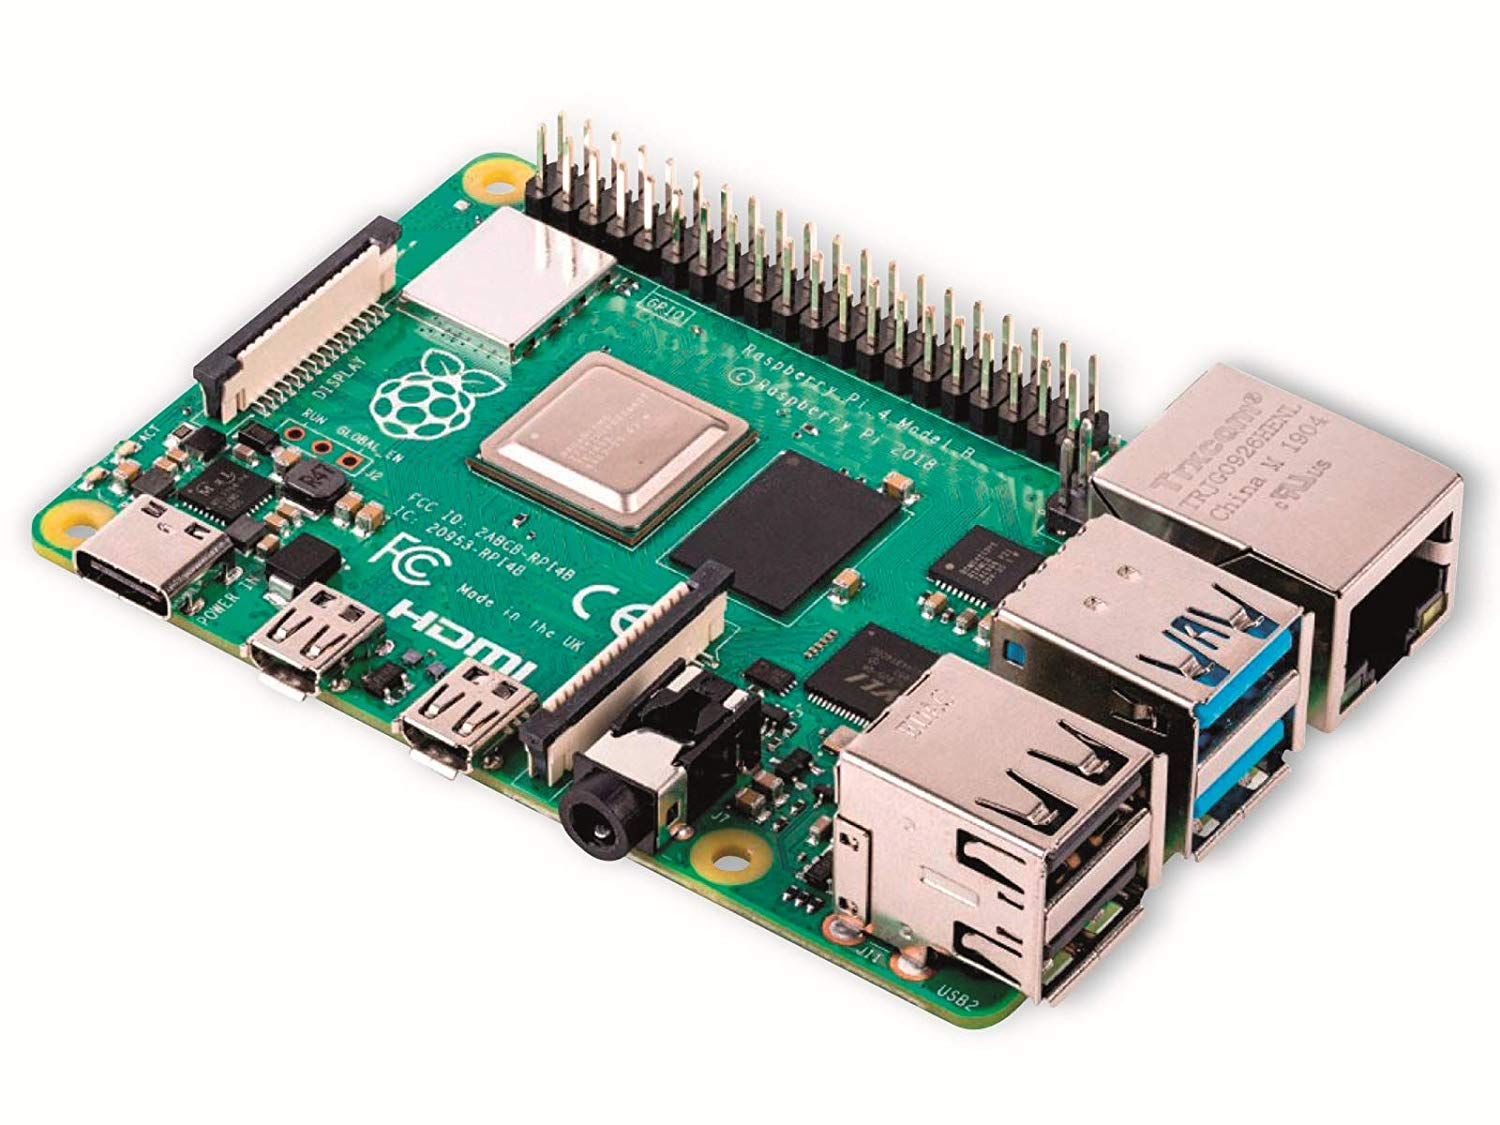
\includegraphics[width=40mm, height=30mm]{raspberry.jpg}
		\end{minipage}  & \begin{minipage}{.2\textwidth}
			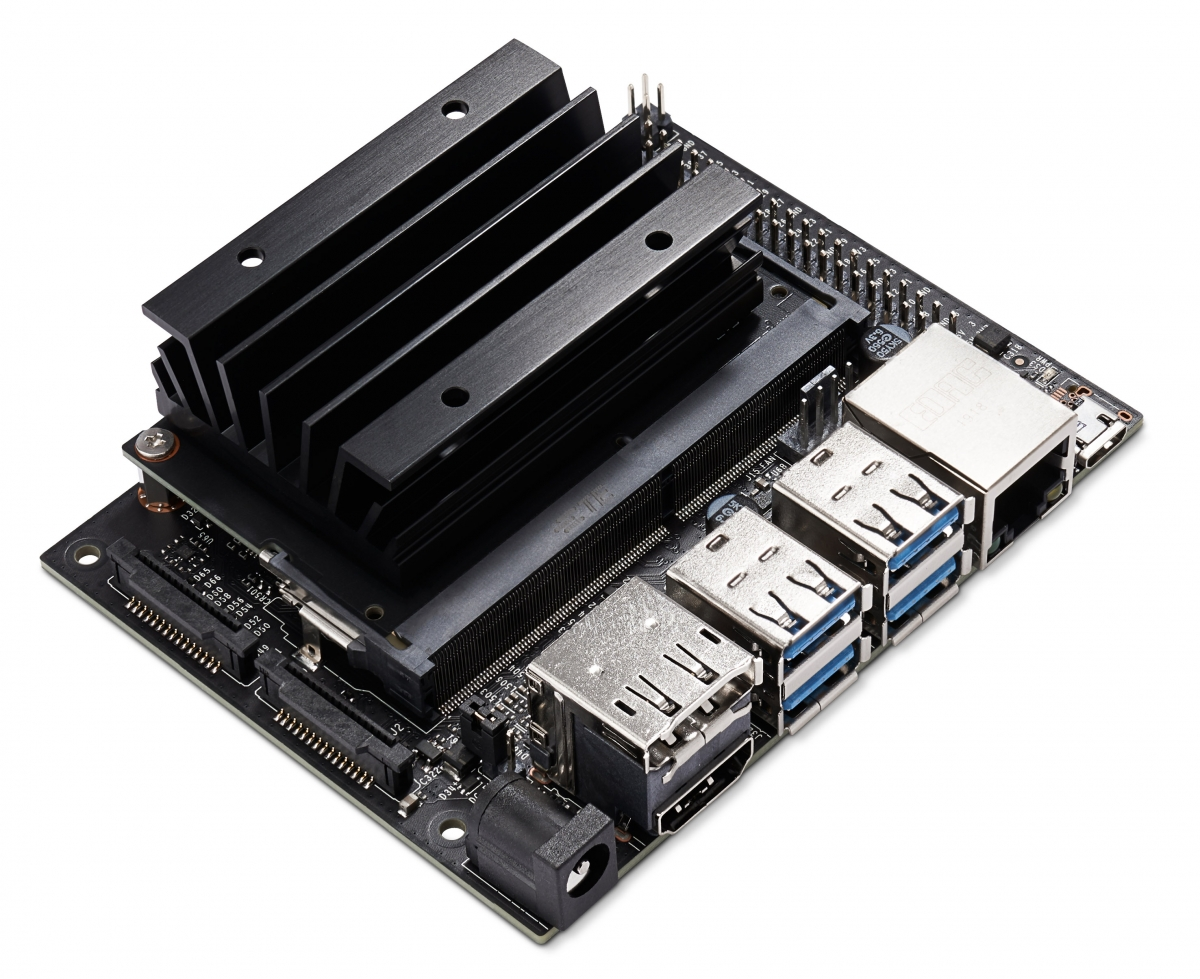
\includegraphics[width=40mm, height=30mm]{jetson.jpg}
		\end{minipage} & \begin{minipage}{.2\textwidth}
			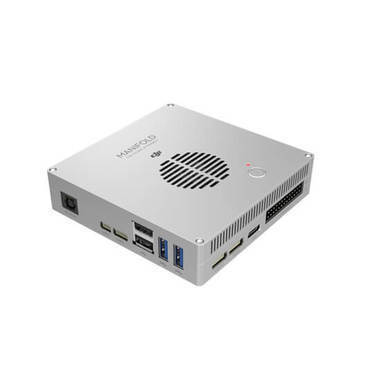
\includegraphics[width=40mm, height=30mm]{manifold.jpg}
		\end{minipage} \\
		\bottomrule
	\end{tabular}
\end{table}

\subsubsection{Power Supply options}
As shown in \cref{tab:power-sources}, there are different options for
the raspberry pi power sources, we have chosen the second option
RPI pack because it is a complete package and lightweight compared 
to other options; availability was also another primary concern. 
\begin{table}[H]
	\centering
	\caption{A comparison of the Power-supply sources for RPI4.}
	\label{tab:power-sources}  
	\begin{tabular}{ p{3cm} p{4cm} p{4cm} p{4cm} }
		\toprule
		\textit{} & \textit{UPS HAT Stable \& Lithium ion battery} & 
		\textit{RPI-ups-pack Lithium polymer battery} & \textit{Power bank}\\ \midrule
				Weight & 80g & 70g & 1.2kg \\ \addlinespace
				Voltage,current & 5V 3.5A  & 5V 3.5A &  5V 3.5A\\ \addlinespace
				
				Price \& Availability & \qar{100}.board available online without batteries & 
				\qar{80}. Available online with battery included & \qar{60}. available 
				locally\\ \addlinespace
				Charging duration  & longer & fast & longer \\ \addlinespace	
				Picture & \begin{minipage}{.2\textwidth}
					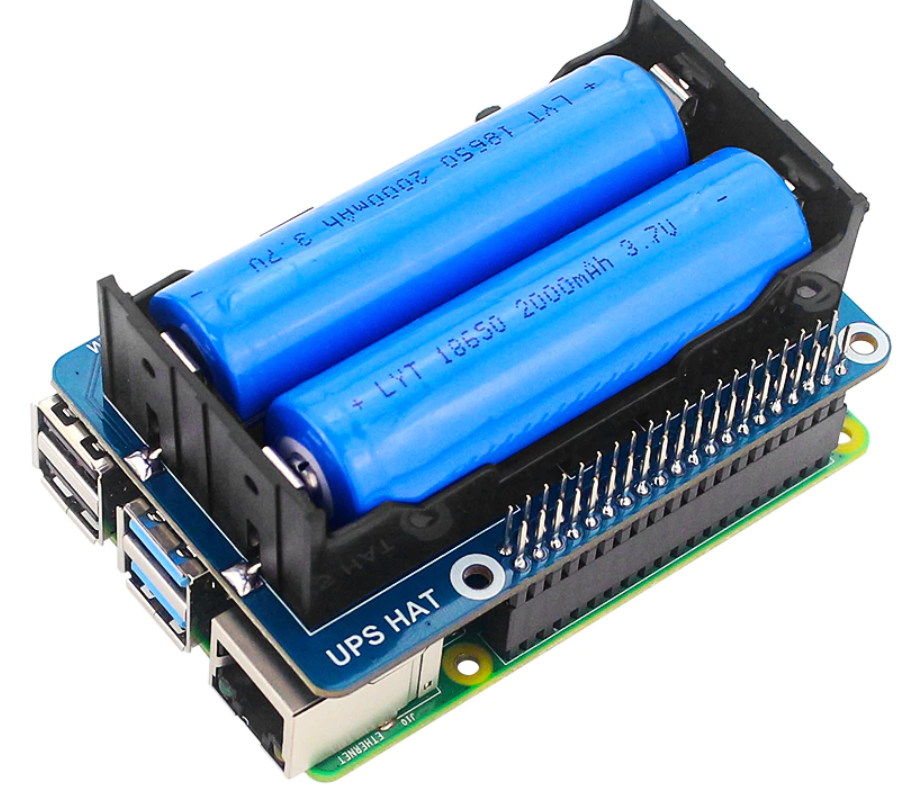
\includegraphics[width=40mm, height=30mm]{ion-battery-ups-haT.png}
				\end{minipage}  & \begin{minipage}{.2\textwidth}
					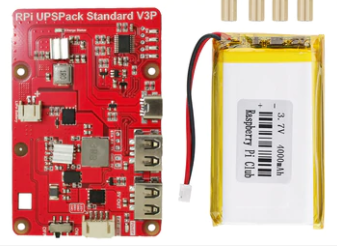
\includegraphics[width=40mm, height=30mm]{rpi-ups-pack.png}
				\end{minipage} & \begin{minipage}{.2\textwidth}
					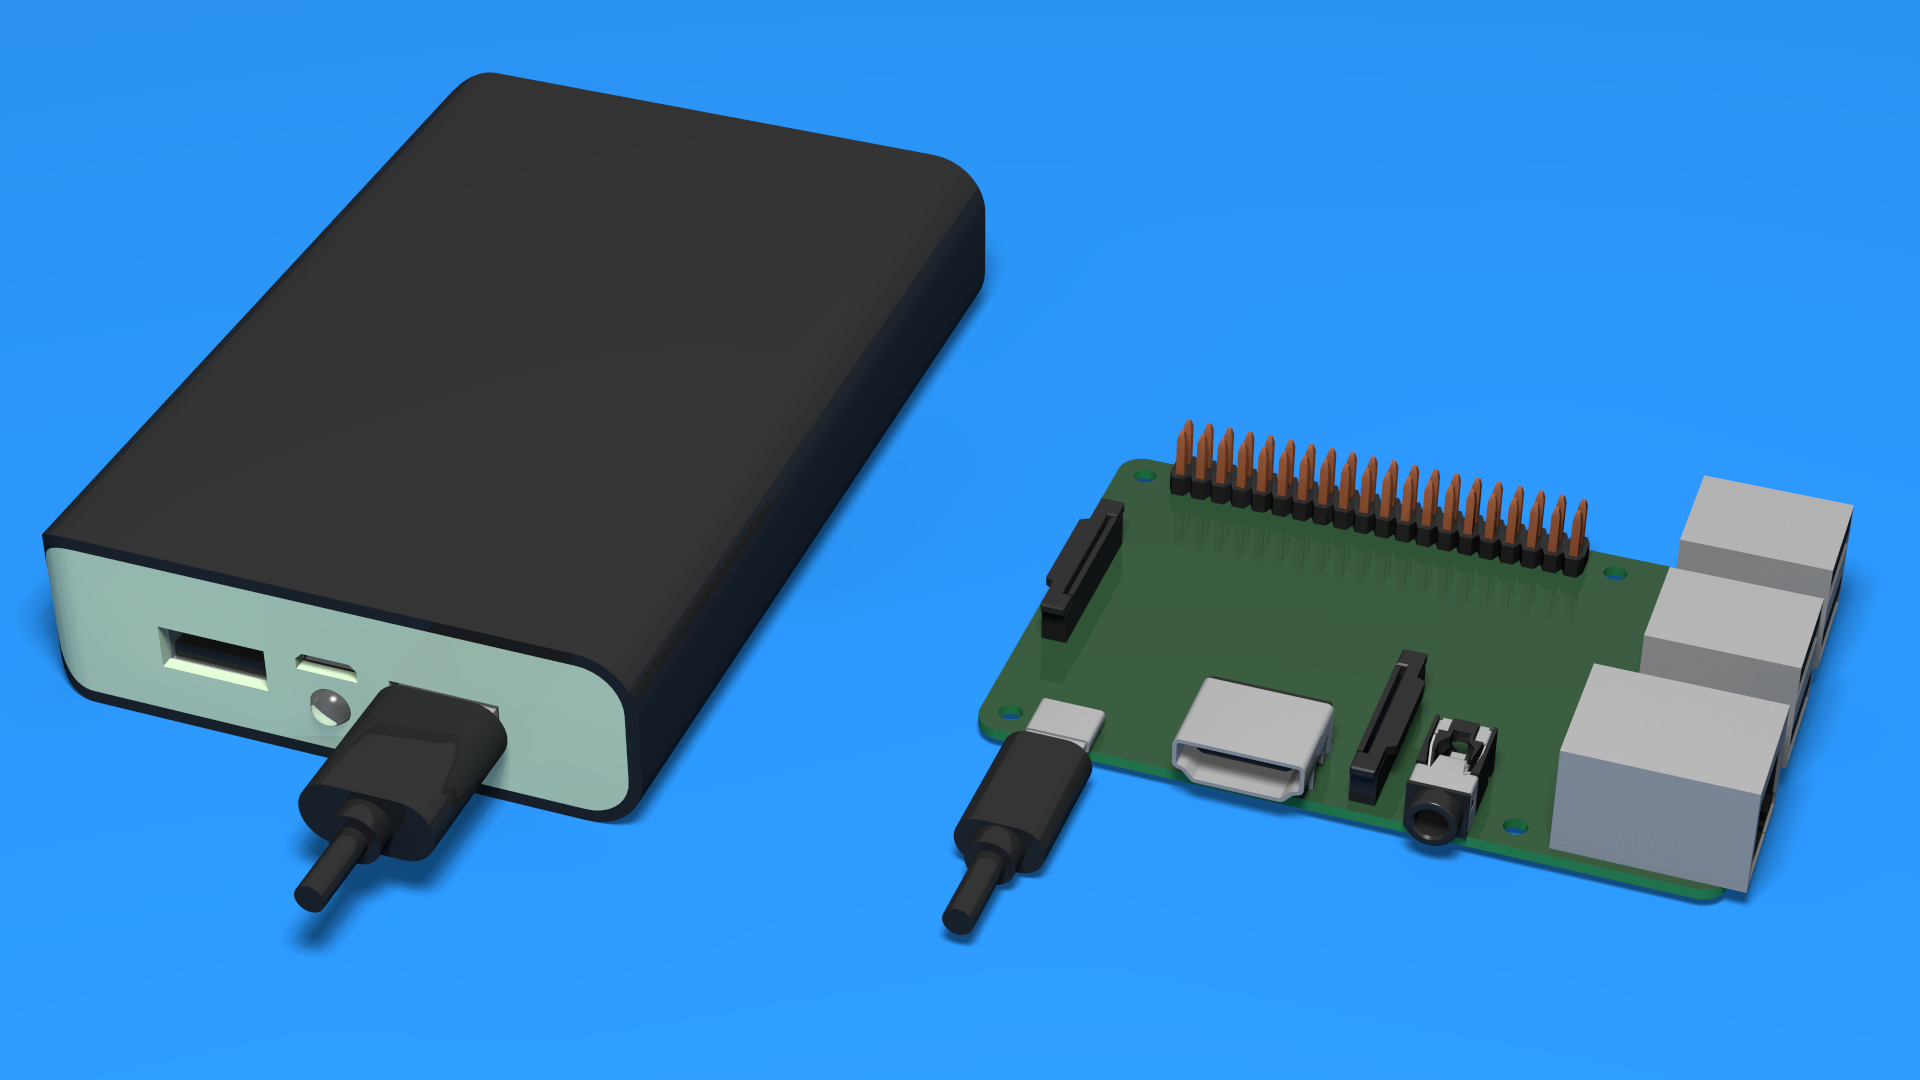
\includegraphics[width=40mm, height=30mm]{power-banks.png}
				\end{minipage} \\
				\bottomrule
			\end{tabular}
		\end{table}


	

\subsection{Software design}

\begin{newrequirements}
    \begin{todolist}
    \item You should document the structural and 
        the behavioral aspects of your software 
        components. For projects that only use 
        embedded code (e.g., programming 
        microprocessor), a flow-chart 
        describing your software design could 
        be sufficient. Projects with user 
        interfaces may elaborate on the 
        functioning of the interface using some 
        of the models mentioned below. 

    \item The software components could be 
        documented using class diagram for the 
        whole system. While Class may be too 
        specific to JAVA or C++ environments, 
        you may use equivalent components 
        applicable to your design. For 
        instance, VI for LabVIEW designs, MDL 
        files in MATLAB, etc… If the model is 
        too big, partition the diagram using 
        some reasonable criteria.  For example, 
        you may provide the entity classes and 
        the controller classes as separate 
        diagrams. 

    \item Specific emphasis should be given to 
        the elaboration of the software 
        components that are responsible for 
        interfacing with the hardware 
        components of your design. For example, 
        if a protocol-like procedure was 
        developed in connecting to a hardware 
        module then it should be explained in 
        detail. Such components may include 
        packetization/depaketization 
        procedures, etc… 

    \item Wherever applicable, all associations 
        between classes/software-modules should 
        be identified through defining the 
        association name and the multiplicities 
        on both ends. Aggregation and 
        inheritance relationships should be 
        identified.  A brief explanation should 
        accompany each diagram. 

    \item Overall software logic may also be 
        described in order to know the 
        appropriate logic flow. In case of 
        LabVIEW or SIMULINK programs, this may 
        not be needed. For other programming 
        environments, the state diagram or 
        extended flow chart may be sufficient. 

    \item In case of graphical codes (such as 
        LabVIEW programs) the software 
        structure may be described by various 
        sub-Vis of the system. Similarly for 
        SIMULINK diagrams, the models should be 
        explained individually. The complete 
        program (graphical/text) should be 
        included in appendix and should not be 
        listed completely in this section. 
                
    \end{todolist}
\end{newrequirements}

\subsubsection{Simulation}

\lipsum[5]

\subsubsection{User Interface}

\lipsum[9]

\end{document}
